%*******************************************************************************************%
%            	DYNAMIC MODELLING AND CONTROL OF BALANCED PARALLEL MECHANISMS           	%
% 																					   		%
% April 26, 2015														 						%
% Authors: Andre G. Coutinho, Tarcisio A. H. Coelho					%
% bash adaptive.sh							 												%
% 																							%
%*******************************************************************************************%



%%%%%%%%%%%%%%%%%%%%%%
\documentclass[a4paper,11pt,brazil,fleqn]{article}
\synctex=1
%%%%%%%%%%%%%%%%%%%%%%

% \usepackage{natbib}
\usepackage[english]{babel}
% \usepackage{amsmath,amssymb,amsthm,amsfonts,textcomp}
% \usepackage{eucal,eufrak,mathrsfs,bbm,stmaryrd}
\usepackage{color}
\usepackage{amsthm}
\usepackage{array,hhline,supertabular}
\usepackage[colorlinks,citecolor=black,urlcolor=black,linkcolor=black]{hyperref}
\usepackage[pdftex]{graphicx}
\usepackage{multicol}
\usepackage[symbol]{footmisc}
\usepackage{enumitem}
\usepackage{float}
\usepackage{titlesec}
\usepackage{nomencl}
\usepackage{EXTRAS/special-char}
\usepackage{EXTRAS/special-conf}
\usepackage{subfigure}

\graphicspath{{FIGURES/}{../FIGURES/}}
\makenomenclature


%%%%%%%%%%%%%%%%%%%%%%
\begin{document}
%%%%%%%%%%%%%%%%%%%%%%

\noindent
{\bf \huge A new approach for designing dynamic balanced serial mechanisms}\\

%Conditions for the decopling of dynamic equations in serial manipulators by applying the adaptive balancing

\noindent
{\Large 		Andr\'e Garnier Coutinho$\,{}^\text{a}$,
			Tarcisio Antonio Hess Coelho$\,{}^\text{b}$
}\\

\noindent
{${}^\text{a}$ \it Department of Mechatronics and Mechanical Systems Engineering, Escola Politecnica, 
University of Sao Paulo, Brazil. E-mail: andre.garnier.coutinho@usp.br}

\noindent
{${}^\text{b}$ \it Department of Mechatronics and Mechanical Systems Engineering, Escola Politecnica, 
University of Sao Paulo, Brazil. E-mail: tarchess@usp.br}

\vspace{24pt}

% \begin{multicols}{1}

\begin{abstract}

Adaptive balancing means that the mechanical structure of the manipulator is modified in order to achieve the decoupling of dynamic equations. This work deals with a systematic methodology for the adaptive balancing. Basically, two balancing techniques are employed here: the addition of counterweight and counter-rotating disks coupled to the moving links. In addition, the feasibility of the dynamic decoupling for 3 distinct types of serial manipulators is discussed regarding the achievement of such balancing and the complexity level of the modified mechanical structure. The balancing conditions are developed for 3-dof spatial and planar open loop-kinematic chain mechanisms, whose topologies are composed of revolute and prismatic joints.

\vspace{10pt}

\noindent
KEYWORDS: {Dynamic balancing, serial mechanisms}
\end{abstract}



\printnomenclature[5em]

% basic mathematical alphabets

\nomenclature[A001]{$a,b, \ldots$}{Scalars, components of column-matrices, components of matrices or indexes}
\nomenclature[A002]{$A,B, \ldots$}{Scalars, components of column-matrices or components of matrices}

\nomenclature[A012]{$\ma, \mb, \ldots$}{Column-matrices}
\nomenclature[A013]{$\mA, \mB, \ldots$}{Matrices}

\nomenclature[A021]{$\va, \vb, \ldots$}{Vectors}
%\nomenclature[A022]{$\vA, \vB, \ldots$}{Tensors}

%\nomenclature[A031]{$\tta, \ttb, \ldots$}{Points}
\nomenclature[A032]{$\ttA, \ttB, \ldots$}{Coordinate systems}

%\nomenclature[A041]{$\llA, \llB, \ldots$}{Rigid bodies or reference frames}

\nomenclature[A051]{$\ssA, \ssB, \ldots$}{Sets or multibody mechanical systems\footnote{
	A multibody mechanical system will be conceived as a set whose elements are 
	material bodies, joints, actuators, energy storage, dissipation and transformation elements
	and a mathematical model (which includes physical parameters, model variables and 
	constitutive, constraint and dynamic equations).
	}}


% special char

%\nomenclature[CAA01]{$a_{n,l}$}{Arbitrary physical parameter}
% \nomenclature[CAA02]{$\nb a_{n,l}$}{Fixed physical parameter}
%\nomenclature[CAA11]{$\mA_{n}$}{Jacobian matrix of kinematic invariants ($\mc_n$) with respect to 
%	quasi-accelerations ($\dot\mp_n$)}
%\nomenclature[CAA21]{$\va_{\ttp \rl \llE}$}{Acceleration of point $\ttp$ measured relatively to reference frame $\llE$}
\nomenclature[CAB01]{$\ttB_i$}{Coordinate system fixed in the i\ts{th} rigid body of the mechanical system}

\nomenclature[CAC01]{$\mC$}{Kinematic constraints matrix}
%\nomenclature[CAC11]{$\mc_{n}$}{Kinematic invariants (constraints) column-matrix}
%\nomenclature[CAC51]{$\ssC^s$}{Differentiability class}
\nomenclature[CAC91]{$\ccos(.)$}{Shorthand notation for $\cos(.)$}

%\nomenclature[CAD11]{$\md_{n}$}{Dynamic invariants column-matrix}
%\nomenclature[CAD91]{$\dd$}{Differential operator}
%\nomenclature[CGD91]{$\dl$}{Variation operator}

%\nomenclature[CAF01]{$f_{n,j}$}{Generalized force}
%\nomenclature[CAF11]{$\mf_{n}$}{Generalized forces column-matrix}
%\nomenclature[CAF21]{$\vf_{\llB}$}{Resultant force acting on body $\llB$ (excluding constraint forces)}

%\nomenclature[CAG01]{$g_{n,j}$}{Generalized gyroscopic inertia force}
%\nomenclature[CAG11]{$\mg_{n}$}{Generalized gyroscopic inertia forces column-matrix}

%\nomenclature[CAI21]{$\vI_{\llB \rl \ttp}$}{Inertia tensor of rigid body $\llB$ relative to point $\ttp$}
%\nomenclature[CAI51]{$\ssI_{x}(\ssS_{n})$}{Set of indexes of variables $x_{n,r}$ defined in the model 
%	of system $\ssS_{n}$, i.e., $\ssI_{x}(\ssS_{n}) = \{ r \,\vert\, x_{n,r} \in \ssS_{n} \}$ }
\nomenclature[CAG01]{$g$}{gravitational acceleration}
\nomenclature[CAG11]{$\mg\ssh$}{Generalized gravitational forces column-matrix of a serial mechanism}
\nomenclature[CAG12]{$\mg\ssh_i$}{Generalized gravitational forces column-matrix of a counter-rotating disc}
\nomenclature[CAG13]{$\mg'$}{Generalized uncoupled gravitational forces column-matrix of a serial mechanism coupled with counter-rotating discs}
\nomenclature[CAG14]{${\mg'}\ssh$}{Generalized gravitational forces column-matrix of a serial mechanism coupled with counter-rotating discs}

\nomenclature[CAJ01]{$J_{x_i}, J_{y_i}, J_{z_i}$}{Moments of inertia of the i\ts{th} rigid body of the mechanical system}

\nomenclature[CAL01]{$l_i$}{Length of the i\ts{th} bar of a serial mechanism}
\nomenclature[CAL01]{$l_{g_i}$}{Position of the mass center of the i\ts{th} bar relative to the i\ts{th} joint and of a serial mechanism}

\nomenclature[CAM01]{$m_i$}{Mass of the i\ts{th} rigid body of the mechanical system}
%\nomenclature[CAM21]{$\vm_{\llB \rl \ttp}$}{Resultant moment (torque) acting on body $\llB$ 
%	measured relatively to pole $\ttp$ (excluding constraint moments)}
\nomenclature[CAM11]{$\mM\ssh$}{Generalized inertia matrix of a serial mechanism}
\nomenclature[CAM12]{$\mM\ssh_i$}{Generalized inertia matrix of a counter-rotating disc}
\nomenclature[CAM13]{$\mM'$}{Generalized uncoupled inertia matrix of a serial mechanism coupled with counter-rotating discs}
\nomenclature[CAM14]{${\mM'}\ssh$}{Generalized inertia matrix of a serial mechanism coupled with counter-rotating discs}

\nomenclature[CAN41]{$\llN$}{Inertial reference frame}
%\nomenclature[CGN01]{$\nu_{x}(\ssS_{n})$}{Number of elements of the set $\ssI_{x}(\ssS_{n})$}
%\nomenclature[CGN02]{$\nu\ssh(\ssS_{n})$}{Number of degrees of freedom of the mechanical system $\ssS_{n}$}

%\nomenclature[CAP01]{$p_{n,j}$}{Quasi-velocity}
%\nomenclature[CAP02]{$\dot p_{n,j}$}{Quasi-acceleration}
\nomenclature[CAP11]{$\mp\ssh$}{Independent quasi-velocities column-matrix}
\nomenclature[CAP12]{$\mp^\circ$}{Redundant quasi-velocities column-matrix}
\nomenclature[CAP13]{$\mp$}{Quasi-velocities column-matrix}

\nomenclature[CAQ01]{$q_i$}{Generalized coordinate}
\nomenclature[CAQ11]{$\mq\ssh$}{Independent generalized coordinates column-matrix}

%\nomenclature[CAR21]{$\vr_{\ttp_2 \rl \ttp_1}$}{Position of point $\ttp_2$ relative to point $\ttp_1$}
% \nomenclature[CAR51]{$\ssR^s$}{Set of $s$-tuples of real numbers}

\nomenclature[CAS91]{$\ssin(.)$}{Shorthand notation for $\sin(.)$}

%\nomenclature[CAT01]{$t$}{Time}

\nomenclature[CAU01]{$u_i$}{Effort made by the i\ts{th} actuator of a serial mechanism}
\nomenclature[CAU11]{$\mu$}{Generalized actuators' efforts column-matrix}

%\nomenclature[CAV21]{$\vv_{\ttp \rl \llE}$}{Velocity of point $\ttp$ measured relatively to reference frame $\llE$}

\nomenclature[CAV11]{$\mv\ssh$}{Generalized coupled gyroscopic inertia forces column-matrix of a serial mechanism}
\nomenclature[CAV12]{$\mv\ssh_i$}{Generalized coupled gyroscopic inertia forces column-matrix of a counter-rotating disc}
\nomenclature[CAV13]{$\mv'$}{Generalized uncoupled gyroscopic inertia forces column-matrix of a serial mechanism coupled with counter-rotating discs}
\nomenclature[CAV14]{${\mv'}\ssh$}{Generalized coupled gyroscopic inertia forces column-matrix of a of a serial mechanism coupled with counter-rotating discs}

%\nomenclature[CAW01]{$w_{n,j}$}{Arbitrary term of generalized force or generalized gyroscopic inertia
%	force linear or bilinear with respect to quasi-velocities}
%\nomenclature[CAW11]{$\mw_{n}$}{Column-matrix whose entries are $w_{n,j}$}	
\nomenclature[CGW21]{$\nvct{\vomega_{\scriptscriptstyle i}}_{\ttB_j} $}{Angular velocity of the i\ts{th} rigid body of the mechanical system measured relatively to a inertial reference frame $\llN$, written in the basis of $\ttB_j$}
\nomenclature[CGW31]{$\omega_{x_i}$}{1\ts{st} component of $\nvct{\vomega_{\scriptscriptstyle i}}_{\ttB_i} $}
\nomenclature[CGW32]{$\omega_{y_i}$}{2\ts{nd} component of $\nvct{\vomega_{\scriptscriptstyle i}}_{\ttB_i} $}
\nomenclature[CGW33]{$\omega_{z_i}$}{3\ts{rd} component of $\nvct{\vomega_{\scriptscriptstyle i}}_{\ttB_i} $}

%\nomenclature[CAZ01]{$z_{n,j}$}{Arbitrary term of generalized force or generalized gyroscopic inertia
%	force independent of quasi-velocities}
%\nomenclature[CAZ11]{$\mz_{n}$}{Column-matrix whose entries are $z_{n,j}$}	

\nomenclature[CN011]{$\mzr$}{Null column-matrix or null matrix}
%\nomenclature[CN021]{$\vzr$}{Null vector or null tensor}

\nomenclature[CN111]{$\mone$}{Identity matrix}
\nomenclature[CN112]{$\nvct{\mone}_{\ttB_i \rl \ttB_j} $}{Change of basis matrix, i.e. $\nvct{\vv}_{\ttB_i} = \nvct{\mone}_{\ttB_i \rl \ttB_j} \cdot \nvct{\vv}_{\ttB_j} $ }
%\nomenclature[CN121]{$\vone$}{Identity tensor}


% matrix/vector notations

% \nomenclature[SM001]{$\nvct{x_{r}}$}{Column-matrix defined by the entries $x_{r}$}
% \nomenclature[SM011]{$\nmat{X_{rs}}$}{Matrix defined by the entries $X_{rs}$}
% \nomenclature[SM012]{$\ndmat{x_{r}}$}{Diagonal-matrix representation of $x_{r}$}

% \nomenclature[SM021]{$\nvct{\vw}_{\ttE}$}{Coordinate column-matrix of vector $\vw$
 	% in coordinate system $\ttE$}
% \nomenclature[SM022]{$\nvct{\ttp}_{\ttE}$}{Coordinate column-matrix of point $\ttp$
 	% in coordinate system $\ttE$}
% \nomenclature[SM023]{$\nhvct{\ttp}_{\ttE}$}{Homogeneous coordinates column-matrix of point $\ttp$
 	% in coordinate system $\ttE$} 

% \nomenclature[SM031]{$\nmat{\vZ}_{\ttE' \rl \ttE}$}{Matrix representing tensor $\vZ$
 	% in terms of coordinate systems $\ttE$ and $\ttE'$ (if $\vw'=\vZ \cdot \vw$, then 
 	% $\nvct{\vw'}_{\ttE'}= \nmat{\vZ}_{\ttE' \rl \ttE} \, \nvct{\vw}_{\ttE}$)}
% \nomenclature[SM032]{$\nsmat{\vw}_{\ttE \rl \ttE}$}{Skew-symmetric matrix representation
	% of $\nvct{\vw}_{\ttE}$} 	

\nomenclature[SM101]{$\ntmat{\cdot}$}{Matrix transposition}
%\nomenclature[SM102]{$\nimat{\cdot}$}{Matrix inversion}
%\nomenclature[SM103]{$\nomat{\cdot}$}{Matrix infinity norm}	




%--------------------INTRODUCTION--------------------%

\section{Introduction and literature review}\label{S01}

Balancing is an important issue related to the design of mechanical systems in general, and also serial manipulators, in particular. In fact, the performance of parallel mechanisms associated to specific applications depends on the choice of the balancing method, namely, either static or dynamic, either passive or active, whether it is valid for a given trajectory or even for any motion.

Adaptive balancing means that the mechanical structure of the manipulator is modified in order to achieve the decoupling of dynamic equations. The modifications comprise the addition of either counterweights, or counter-rotating disks or even both to the original kinematic chain of the manipulator. Consequently, the terms associated to gravitational, centripetal and Coriolis efforts are completely eliminated from the dynamic equations. As a matter of fact, the effective inertias for all the actuator axes are constant and the mathematical expressions of the driving torques/forces become rather simple. One of the main advantages of this approach concerns the reduction of computing time for a closed-loop control of manipulators. Such reduction is really significant and it constitutes in a great benefit for real-time applications.

The contributions of this work are the following: to present a systematic methodology for the adaptive balancing, to discuss the feasibility of the dynamic decoupling for 3 distinct types of serial manipulators, not only in terms of the possibility to achieve such balancing but also in terms of the increase in the complexity level of the modified mechanical structure. The analysed manipulators correspond to 3-dof spatial and planar open loop-kinematic chain, whose topologies are composed of revolute and prismatic joints.

This work is organized as follows. Section 2 describes the proposed methodology, while section 3 deals with the application of the methodology to 3 types of serial manipulators. Finally, the conclusions are drawn in section 4.


%--------------------METHODOLOGY--------------------%

\section{Mothodology}\label{S02}

\subsection{Dynamic Model}\label{S02-1}

O modelo din\^{a}mico de um mecanismo serial pode ser escrito da seguinte maneira:
\begin{equation}
\mM\ssh (\mq\ssh) \ddot{\mq}\ssh + \mv\ssh(\mq\ssh,\dot{\mq}\ssh) + \mg\ssh (\mq\ssh) = \mu
\end{equation}

Sendo $\mq\ssh$ um conjunto de coordenadas generalizadas independentes, cujos elementos s\~{a}o os deslocamentos relativos das juntas e $\mu$ os esfor\c{c}os generalizados nas dire\c{c}\~oes das quasi-velocidades independentes $\mp\ssh = \dot{\mq}\ssh$.

Para realizar o balanceamento din\^{a}mico de um mecanismo serial, utilizando abordagem proposta, \'{e} necess\'{a}rio primeiro obter o modelo do mecanismo desbalanceado. Como em um mecanismo serial \'{e} poss\'{i}vel de expressar todas as velocidades lineares absolutas dos centros de massa das barras e todas as velocidades angulares absolutas das barras em fun\c{c}\~ao de $\mq\ssh$ e  $\dot{\mq}\ssh$, o modelo din\^{a}mico pode ser obtido sem grandes dificuldades utilizando m\'{e}todos de mec\'{a}nica anal\'{i}tica, como Lagrange, Kane e Orsino, aliados a programas ou bibliotecas de linguagens de programa\c{c}\~{a}o que s\~{a}o capazes de utilizar manipula\c{c}\~{a}o simb\'{o}lica, como o Mathematica e o SymPy.


\subsection{Static Balancing}\label{S02-2}

Depois de obtido o modelo din\^{a}mico, realiza-se o balanceamento est\'{a}tico encontrando as posi\c{c}\~{o}es dos centros de massa das barras que fazem com que $\mg\ssh = \mzr$. Isso \'{e} poss\'{i}vel para mecanismos com juntas apenas rotativas e mecanismos com juntas prism\'{a}ticas cujas dire\c{c}\~{o}es s\~{a}o ortogonais \`{a} gravidade. O posicionamento dos centros de massa \'e realizado mecanicamente com o prologamento das barras do mecanismo e adi\c{c}\~ao de contra-pesos.

\subsection{Dynamic Balancing}\label{S02-3}

O balanceamento din\^{a}mico \'{e} obtido acoplando discos girantes ao modelo do mecanismo est\'{a}ticamente balanceado. Isso \'{e} feito utilizando a t\'{e}cnica de acoplamento de subsistemas do M\'{e}todo Orsino.

Seja $\ssM_0$ um subsistema mec\^anico constituido por um mecanismo serial estaticamente balanceado, cuja equa\c{c}\~{a}o de movimento \'e dada pela equa\c{c}\~{a}o (1), com $\mg\ssh = \mzr$. Seja $\ssM_i$ um subsistema mec\^anico constituido de um disco girante que ser\'a acoplado ao mecanismo, cuja equa\c{c}\~{a}o de movimento \'e dada por:
\begin{equation}
\mM\ssh_i \dot{\mp}\ssh + \mv\ssh_i + \mg\ssh_i = \mu_i
\end{equation}
Sendo $\mp\ssh$ um conjunto de quasi-velocidades independentes, cujos elementos s\~{a}o as componentes n\~{a}o nulas do vetor velocidade angular absoluta do disco, escrito em uma base solid\'{a}ria ao disco, e $\mv\ssh_i = \mg\ssh_i = \mu_i = \mzr$. Nesse modelo, s\~ao considerados apenas os efeitos das in\'{e}rcias rotativas, sendo os efeitos da massa do disco considerados na massa e nos momentos de in\'{e}rcia da barra em que o disco for acoplado, efetando tamb\'{e}m no c\'{a}lculo do posicionamento dos contra-pesos, de modo que o mecanismo continue est\'{a}ticamente balanceado.

Supondo que ir\~{a}o ser acoplados $n$ discos ao mecanismo, s\~ao feitas as seguintes defini\c{c}\~oes:

\begin{equation}
\mM' =
\begin{bmatrix}
\mM\ssh &  \mzr  & \ldots & \mzr\\
\mzr  &  \mM\ssh_1 & \ldots & \mzr\\
\vdots & \vdots & \ddots & \vdots\\
\mzr  &   \mzr       &\ldots & \mM\ssh_{n}
\end{bmatrix}
\end{equation}
\begin{equation}
\mv' = \begin{bmatrix}
{\mv\ssh}^\msT & {\mv\ssh_1}^\msT & ... & {\mv\ssh_{n}}^\msT
\end{bmatrix}^\msT
\end{equation}
\begin{equation}
\mg' = \begin{bmatrix}
{\mg\ssh}^\msT & {\mg\ssh_1}^\msT & ... & {\mg\ssh_{n}}^\msT
\end{bmatrix}^\msT
\end{equation}
\begin{equation}
\mp^\circ = \begin{bmatrix}
{\mp\ssh_1}^\msT & ... & {\mp\ssh_{n}}^\msT
\end{bmatrix}^\msT
\end{equation}
\begin{equation}
\mp = \begin{bmatrix}
{\mp\ssh}^\msT & {\mp^\circ}^\msT
\end{bmatrix}^\msT
\end{equation}

Seja $\underline{\mp}^\circ$ o vetor $\mp^\circ$ escrito em fun\c{c}\~{a}o de $\mq\ssh$ e $\mp\ssh$, ou seja:

\begin{equation}
\mp^\circ = \underline{\mp}^\circ(\mq\ssh, \mp\ssh) 
\end{equation}

Definimos a seguinte matriz das restri\c{c}\~{o}es cinem\'{a}ticas:

\begin{equation}
\mC =
\begin{bmatrix}
\mone \\
\displaystyle\frac{\partial \underline{\mp}^\circ}{\partial \mp\ssh}
\end{bmatrix}
\end{equation}

O modelo din\^{a}mico do mecanismo serial com os discos acoplados, \'{e} dado por:
\begin{equation}
{\mM'}\ssh (\mq\ssh) \ddot{\mq}\ssh + {\mv'}\ssh(\mq\ssh,\dot{\mq}\ssh) + {\mg'}\ssh (\mq\ssh) = \mu
\end{equation}

Sendo:
\begin{equation}
{\mM'}\ssh = \mC^\msT \mM' \mC
\end{equation}
\begin{equation}
{\mv'}\ssh = \mC^\msT ( \mM' \dot{\mC} \dot{\mq}\ssh + \mv')
\end{equation}
\begin{equation}
{\mg'}\ssh = \mC^\msT \mg'
\end{equation}

O balanceamento din\^{a}mico \'{e} obtido encontrando as rela\c{c}\~{o}es entre os par\^{a}metros do sistema que tornam a matriz ${\mM'}\ssh$ diagonal e o vetor ${\mv'}\ssh$ nulo.


 
%--------------------EXAMPLE---------------------%

\section{Applying the technique}\label{S03}

Nesta se\c{c}\~{a}o, a metodologia proposta ser\'{a} aplicada em tr\^{e}s diferentes mecanismos seriais de 3 graus de liberdade, um plano e dois espaciais. Para isso, primeiramente faremos algumas defini\c{c}\~{o}es v\'{a}lidas para os mecanismos em quest\~{a}o:

\begin{equation}
\mM\ssh = 
\begin{bmatrix}
D_{11} & D_{12} & D_{13} \\
D_{12} & D_{22} & D_{23} \\
D_{13} & D_{23} & D_{33} \\
\end{bmatrix}
\end{equation}
\begin{equation}
\mv\ssh = 
\begin{bmatrix}
D_{111} & D_{122} & D_{133} \\
D_{211} & D_{222} & D_{233} \\
D_{311} & D_{322} & D_{333} \\
\end{bmatrix}
\begin{bmatrix}
\dot{q}_1^2 \\
\dot{q}_2^2 \\
\dot{q}_3^2 \\
\end{bmatrix}
+
2\begin{bmatrix}
D_{112} & D_{113} & D_{123} \\
D_{212} & D_{213} & D_{223} \\
D_{312} & D_{313} & D_{323} \\
\end{bmatrix}
\begin{bmatrix}
\dot{q}_1 \dot{q}_2 \\
\dot{q}_1 \dot{q}_3 \\
\dot{q}_2 \dot{q}_3 \\
\end{bmatrix}
\end{equation}
\begin{equation}
\mg\ssh =
\begin{bmatrix}
D_1 &
D_2 &
D_3
\end{bmatrix}^\top
\end{equation}
\begin{equation}
\mq\ssh =
\begin{bmatrix}
q_1 &
q_2 &
q_3
\end{bmatrix}^\top
\end{equation}
\begin{equation}
\mu =
\begin{bmatrix}
u_1 &
u_2 &
u_3
\end{bmatrix}^\top
\end{equation}

Para juntas rotativas definimos $q_i = \theta_i$ e $u_i = \tau_i$, e para juntas prism\'{a}ticas definimos $q_i = d_i$ and $u_i = f_i$, para ficar de acordo com as nota\c{c}\~{o}es mais tradicionais dessa \'{a}rea.

\subsection{3-DOF RRR planar serial mechanism}\label{S03-1}

\begin{figure}[H]
	\centering
	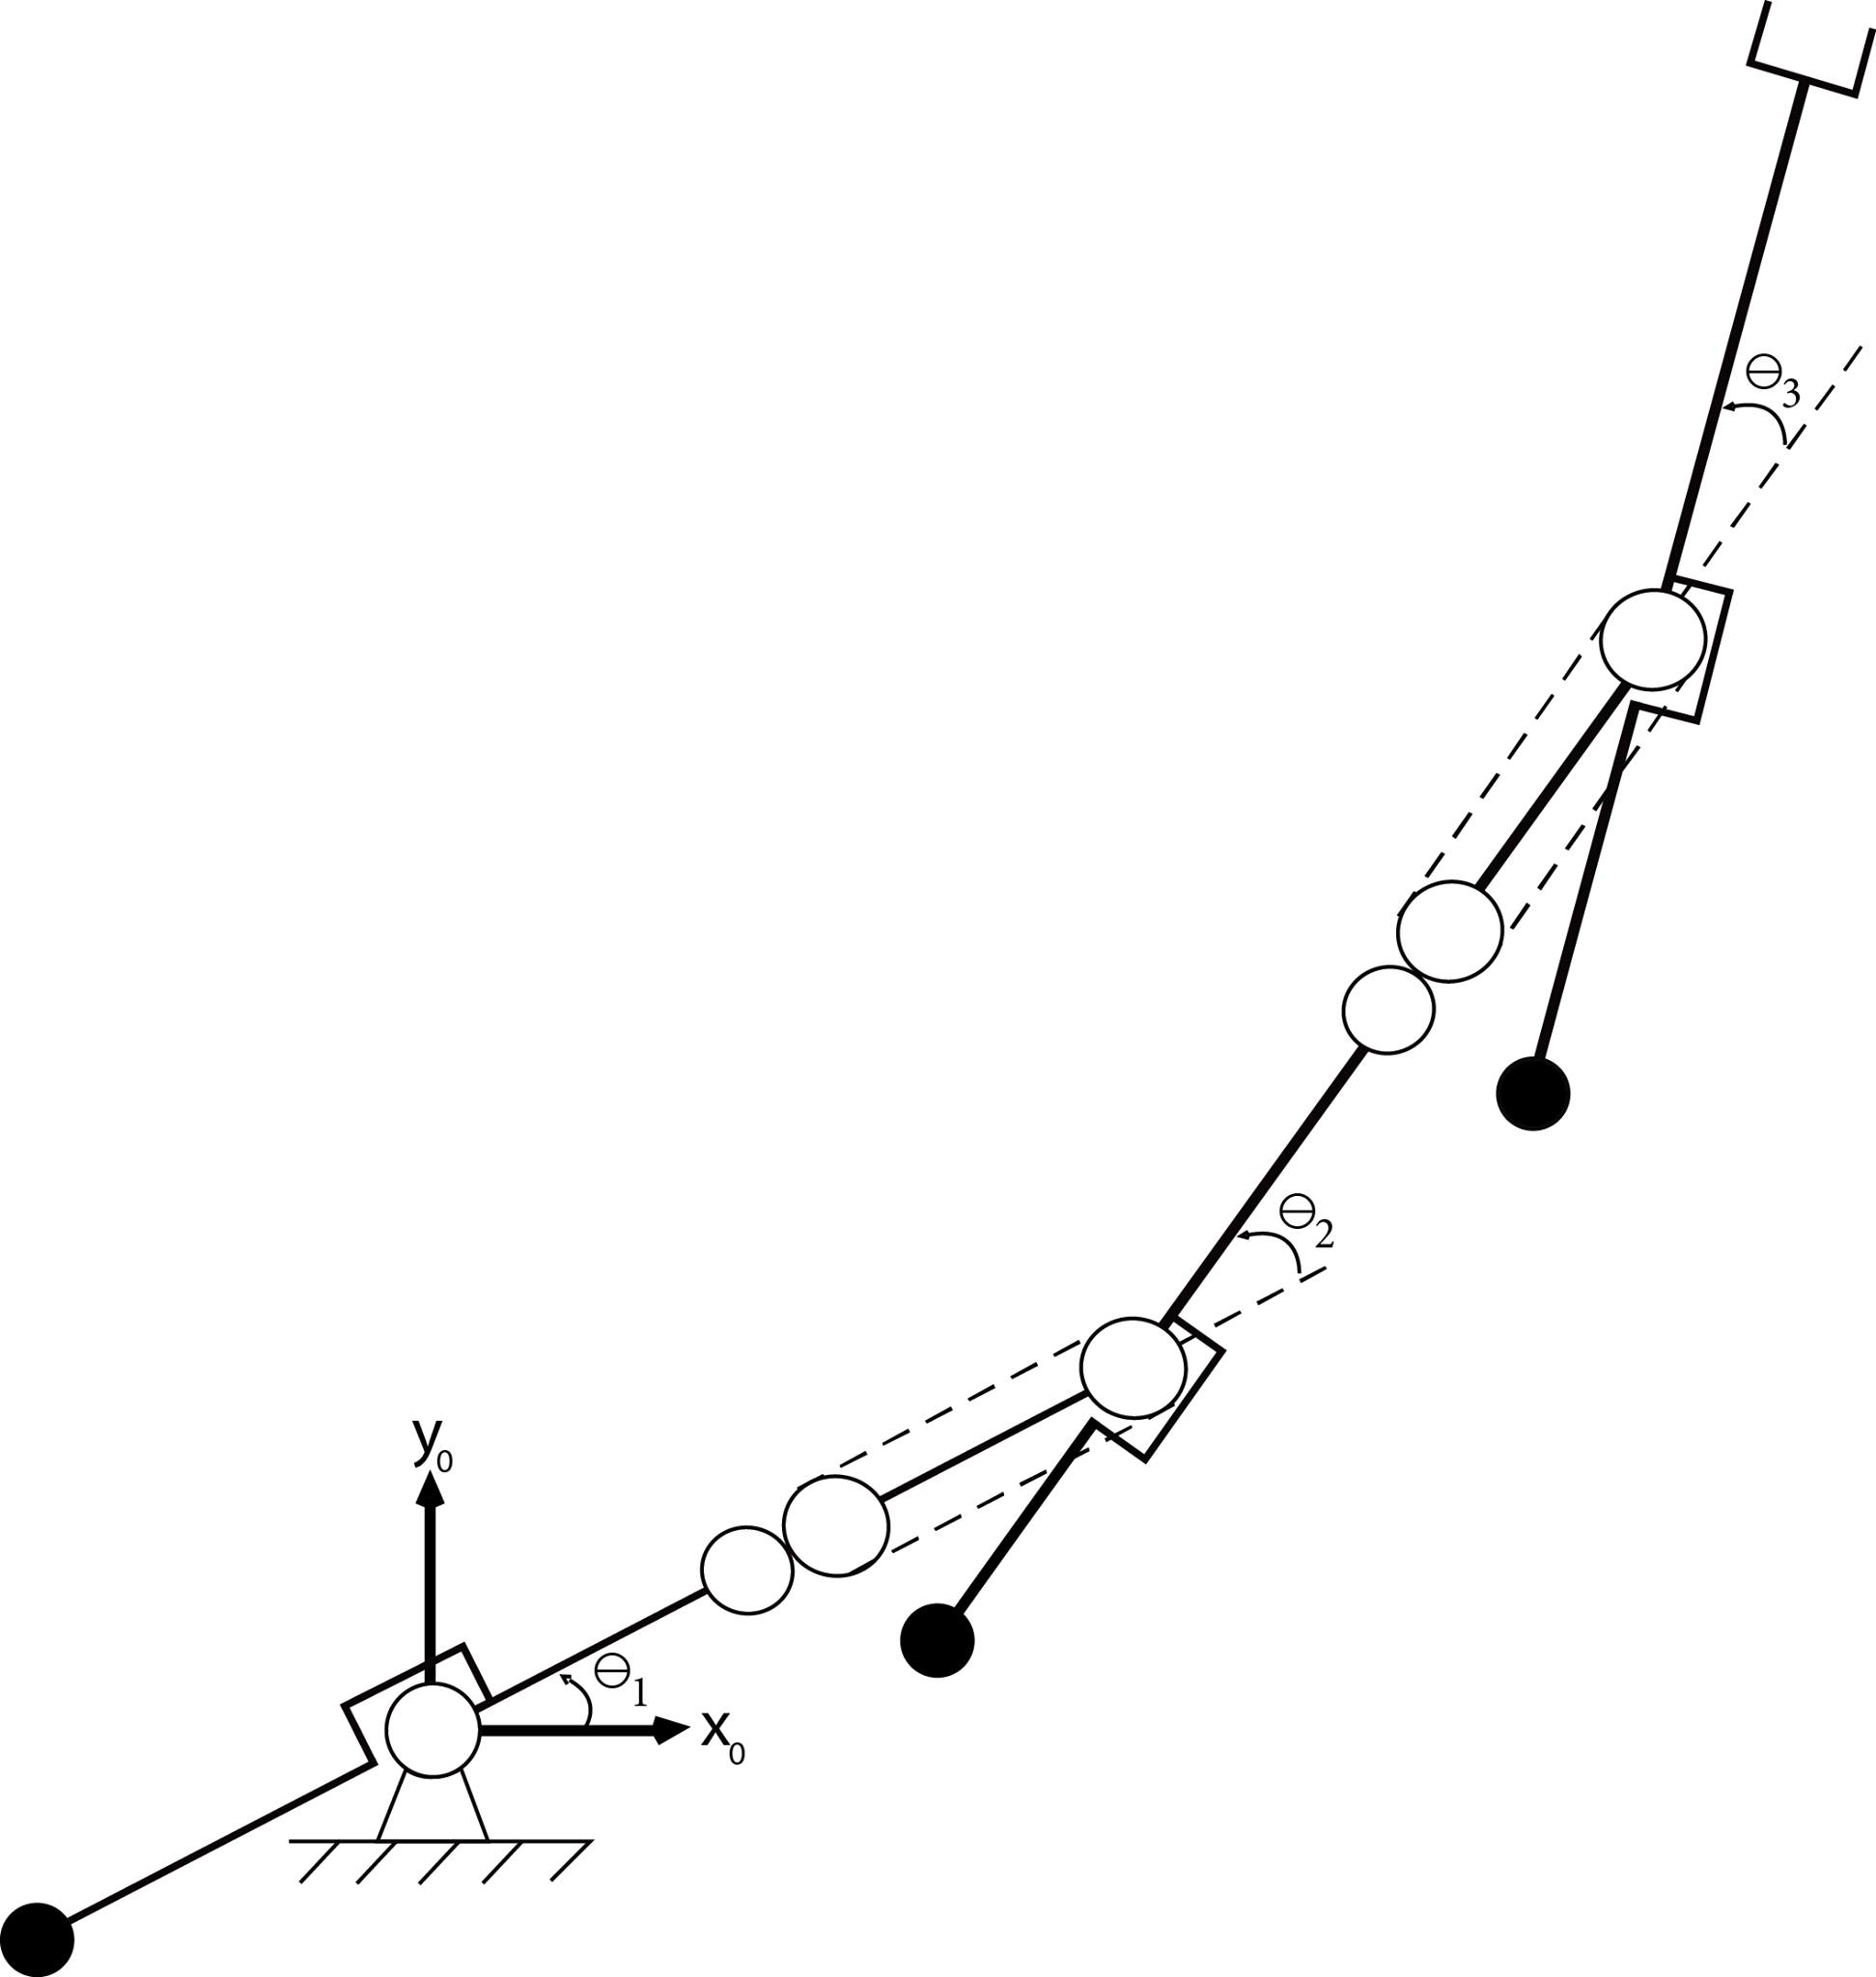
\includegraphics[scale=0.11]{RRR2D.jpg}  
	\caption{Mecanismo RRR plano}
	\label{fig:RRR2D}
\end{figure}

As componentes de $\mg\ssh$ para o mecanismo em quest\~{a}o desbalanceado s\~{a}o dadas por:
\begin{equation}
\begin{cases}
D_1 = g[ (m_1 l_{g_1} + m_2 l_1 + m_3 l_1 ) \ccos(\theta_1) + (m_2 l_{g_2} + m_3 l_2) \ccos(\theta_1 + \theta_2) + m_3 l_{g_3} \ccos(\theta_1 + \theta_2 + \theta_3) ] \\
D_2 = g[  (m_2 l_{g_2} + m_3 l_2) \ccos(\theta_1 + \theta_2) + m_3 l_{g_3} \ccos(\theta_1 + \theta_2 + \theta_3) ] \\
D_3 = g[   m_3 l_{g_3} \ccos(\theta_1 + \theta_2 + \theta_3) ] \\
\end{cases}
\end{equation} 
Realizando o balanceamento est\'{a}tico, temos:
\begin{equation}
\begin{cases}
D_1 = 0 \\
D_2 = 0 \\
D_3 = 0 \\
\end{cases}
\Rightarrow
\begin{cases}
l_{g_1} = -\frac{l_1(m_2 + m_3)}{m_1} \\
l_{g_2} = -\frac{l_2 m_3}{m_2} \\
l_{g_3} = 0 \\
\end{cases}
\end{equation}
Substituindo (20) no modelo do mecanismo, obtemos o modelo din\^{a}mico do mecanismo estaticamente balanceado:
\begin{equation}
\begin{cases}
D_{11} = J_{x_1} + J_{x_2} + J_{x_3} + m_2 l_1^2 + m_3 (l_1^2 + l_2^2) + \frac{l_1^2 (m_2 + m_3)^2}{m_1} + \frac{l_2^2 m_3^2}{m_2} \\
D_{22} = J_{x_2} + J_{x_3} + m_3 l_2^2 + \frac{l_2^2 m_3^2}{m_2} \\
D_{33} = J_{x_3} \\
D_{12} = D_{22} \\
D_{13} = D_{23} = D_{33} \\
\mv\ssh = \mzr \\
\mg\ssh = \mzr
\end{cases}
\end{equation}
Para realizar o balanceamento din\^{a}mico, acoplamos 4 discos ao mecanismo, assim como \'{e} mostrado na figura 1. Como os discos giram em apenas um plano, utilizamos os seguintes modelos din\^{a}micos para eles:
\begin{equation}
\mM\ssh_i = \begin{bmatrix} J_{x_{i+3}} \end{bmatrix}; \; \mp\ssh_i = \begin{bmatrix} \omega_{x_{i+3}} \end{bmatrix}, \; i = 1, 2, 3, 4
\end{equation}
Os discos 1 e 2 est\~{a}o acoplados \`{a} barra 1, sendo que o disco 1 apresenta um giro de $\theta_2$ relativo \`{a} barra 1, devido \`{a} transmiss\~{a}o por correia do giro do motor 2, enquanto o disco 2 apresenta um giro de $\beta\theta_2$, com $\beta < 0$, relativo \'{a} barra 1, devido \'{a} transmiss\~{a}o por engrenagem do giro do disco 1.

Os discos 3 e 4 est\~{a}o acoplados \`{a} barra 2, sendo que o disco 3 apresenta um giro de $\theta_3$ relativo \`{a} barra 2, devido \`{a} transmiss\~{a}o por correia do giro do motor 3, enquanto o disco 4 apresenta um giro de $\gamma\theta_3$, com $\gamma < 0$, relativo \'{a} barra 2, devido \'{a} transmiss\~{a}o por engrenagem do giro do disco 3.

Sendo assim, obtemos os seguintes v\'{i}nculos de quasi-velocidades:
\begin{equation}
\begin{cases}
\omega_{x_4} = \omega_{x_1} + \dot{\theta}_2 \\
\omega_{x_5} = \omega_{x_1} + \beta\dot{\theta}_2 \\
\omega_{x_6} = \omega_{x_2} + \dot{\theta}_3 \\
\omega_{x_7} = \omega_{x_2} + \gamma\dot{\theta}_3 \\
\end{cases}
\Rightarrow
\begin{cases}
\omega_{x_4} = \dot{\theta}_1 + \dot{\theta}_2 \\
\omega_{x_5} = \dot{\theta}_1 + \beta\dot{\theta}_2 \\
\omega_{x_6} = \dot{\theta}_1 + \dot{\theta}_2 + \dot{\theta}_3 \\
\omega_{x_7} = \dot{\theta}_1 + \dot{\theta}_2 + \gamma\dot{\theta}_3 \\
\end{cases}
\Rightarrow
\underline{\mp}^\circ = 
\begin{bmatrix}
\dot{\theta}_1 + \dot{\theta}_2 \\
\dot{\theta}_1 + \beta\dot{\theta}_2 \\
\dot{\theta}_1 + \dot{\theta}_2 + \dot{\theta}_3 \\
\dot{\theta}_1 + \dot{\theta}_2 + \gamma\dot{\theta}_3 \\
\end{bmatrix}
\end{equation}
\begin{equation}
\therefore\mC =
\begin{bmatrix}
\mone \\
\displaystyle\frac{\partial \underline{\mp}^\circ}{\partial \mp\ssh}
\end{bmatrix}  =
\begin{bmatrix}
1 & 0 & 0 \\
0 & 1 & 0 \\
0 & 0 & 1 \\
1 & 1     & 0 \\
1 & \beta & 0 \\
1 & 1     & 1 \\
1 & 1     & \gamma \\
\end{bmatrix} 
\end{equation}
Aplicando as equa\c{c}\~{o}es (?), (?) e (?), obtemos o modelo do mecanismo estaticamente balanceado com os discos acoplados:
\begin{equation}
\begin{cases}
D'_{11} = D_{11} + J_{x_4} + J_{x_5} + J_{x_6} + J_{x_7} \\
D'_{22} = D_{22} + J_{x_4} + J_{x_5} \beta^2 + J_{x_6} + J_{x_7} \\
D'_{33} = D_{33} + J_{x_6} + J_{x_7} \gamma^2 \\
D'_{12} = D_{12} + J_{x_4} + J_{x_5} \beta + J_{x_6} + J_{x_7} \\
D'_{13} = D_{13} + J_{x_6} + J_{x_7} \gamma  \\
D'_{23} = D'_{13}\\
{\mv'}\ssh = \mzr \\
\end{cases}
\end{equation}
Para realizar o balanceamento din\^{a}mico, encontramos os valores de $\beta$ e $\gamma$ em fun\c{c}\~{a}o dos par\^ametros do mecanismo que tornam a matriz ${\mM'}\ssh$ diagonal. Assim, temos:
\begin{equation}
\begin{cases}
D'_{12} = 0 \\
D'_{13} = 0 \\
\end{cases}
\Rightarrow
\begin{cases}
\beta = -\frac{J_{x_2} + J_{x_3} + J_{x_4} + J_{x_6} + J_{x_7} + m_3 l_2^2 + \frac{m_3^2 l_2^2}{m_2}}{J_{x_5}} \\
\gamma = -\frac{J_{x_3} + J_{x_6}}{J_{x_7}} \\
\end{cases}
\end{equation}
Substituindo (26) em (25), obtemos o modelo do mecanismo din\^{a}micamente balanceado:
\begin{equation}
\begin{cases}
\tau_1 = k_1 \ddot{\theta}_1 \\
\tau_2 = k_2 \ddot{\theta}_2 \\
\tau_3 = k_3 \ddot{\theta}_3 \\
\end{cases}
\end{equation}
Sendo:
\begin{equation}
\begin{cases}
k_1 = J_{x_1} + J_{x_2} + J_{x_3} + J_{x_4} + J_{x_5} + J_{x_6} + J_{x_7} + m_2 l_1^2 + m_3 (l_1^2 + l_2^2) + \frac{l_1^2 (m_2 + m_3)^2}{m_1} + \frac{l_2^2 m_3^2}{m_2} \\
k_2 = J_{x_2} + J_{x_3} + J_{x_4} + J_{x_6} + J_{x_7} + m_3 l_2^2 + \frac{l_2^2 m_3^2}{m_2} + \frac{\big(J_{x_2} + J_{x_3} + J_{x_4} + J_{x_6} + J_{x_7} + m_3 l_2^2 + \frac{m_3^2 l_2^2}{m_2}\big)^2}{J_{x_5}} \\
k_3 = \frac{(J_{x_3}+J_{x_6})(J_{x_3}+J_{x_6}+J_{x_7})}{J_{x_7}} \\
\end{cases}
\end{equation}

\subsection{3-DOF RRR spatial serial mechanism} \label{S03-2}

\begin{figure}[H]
	\centering
	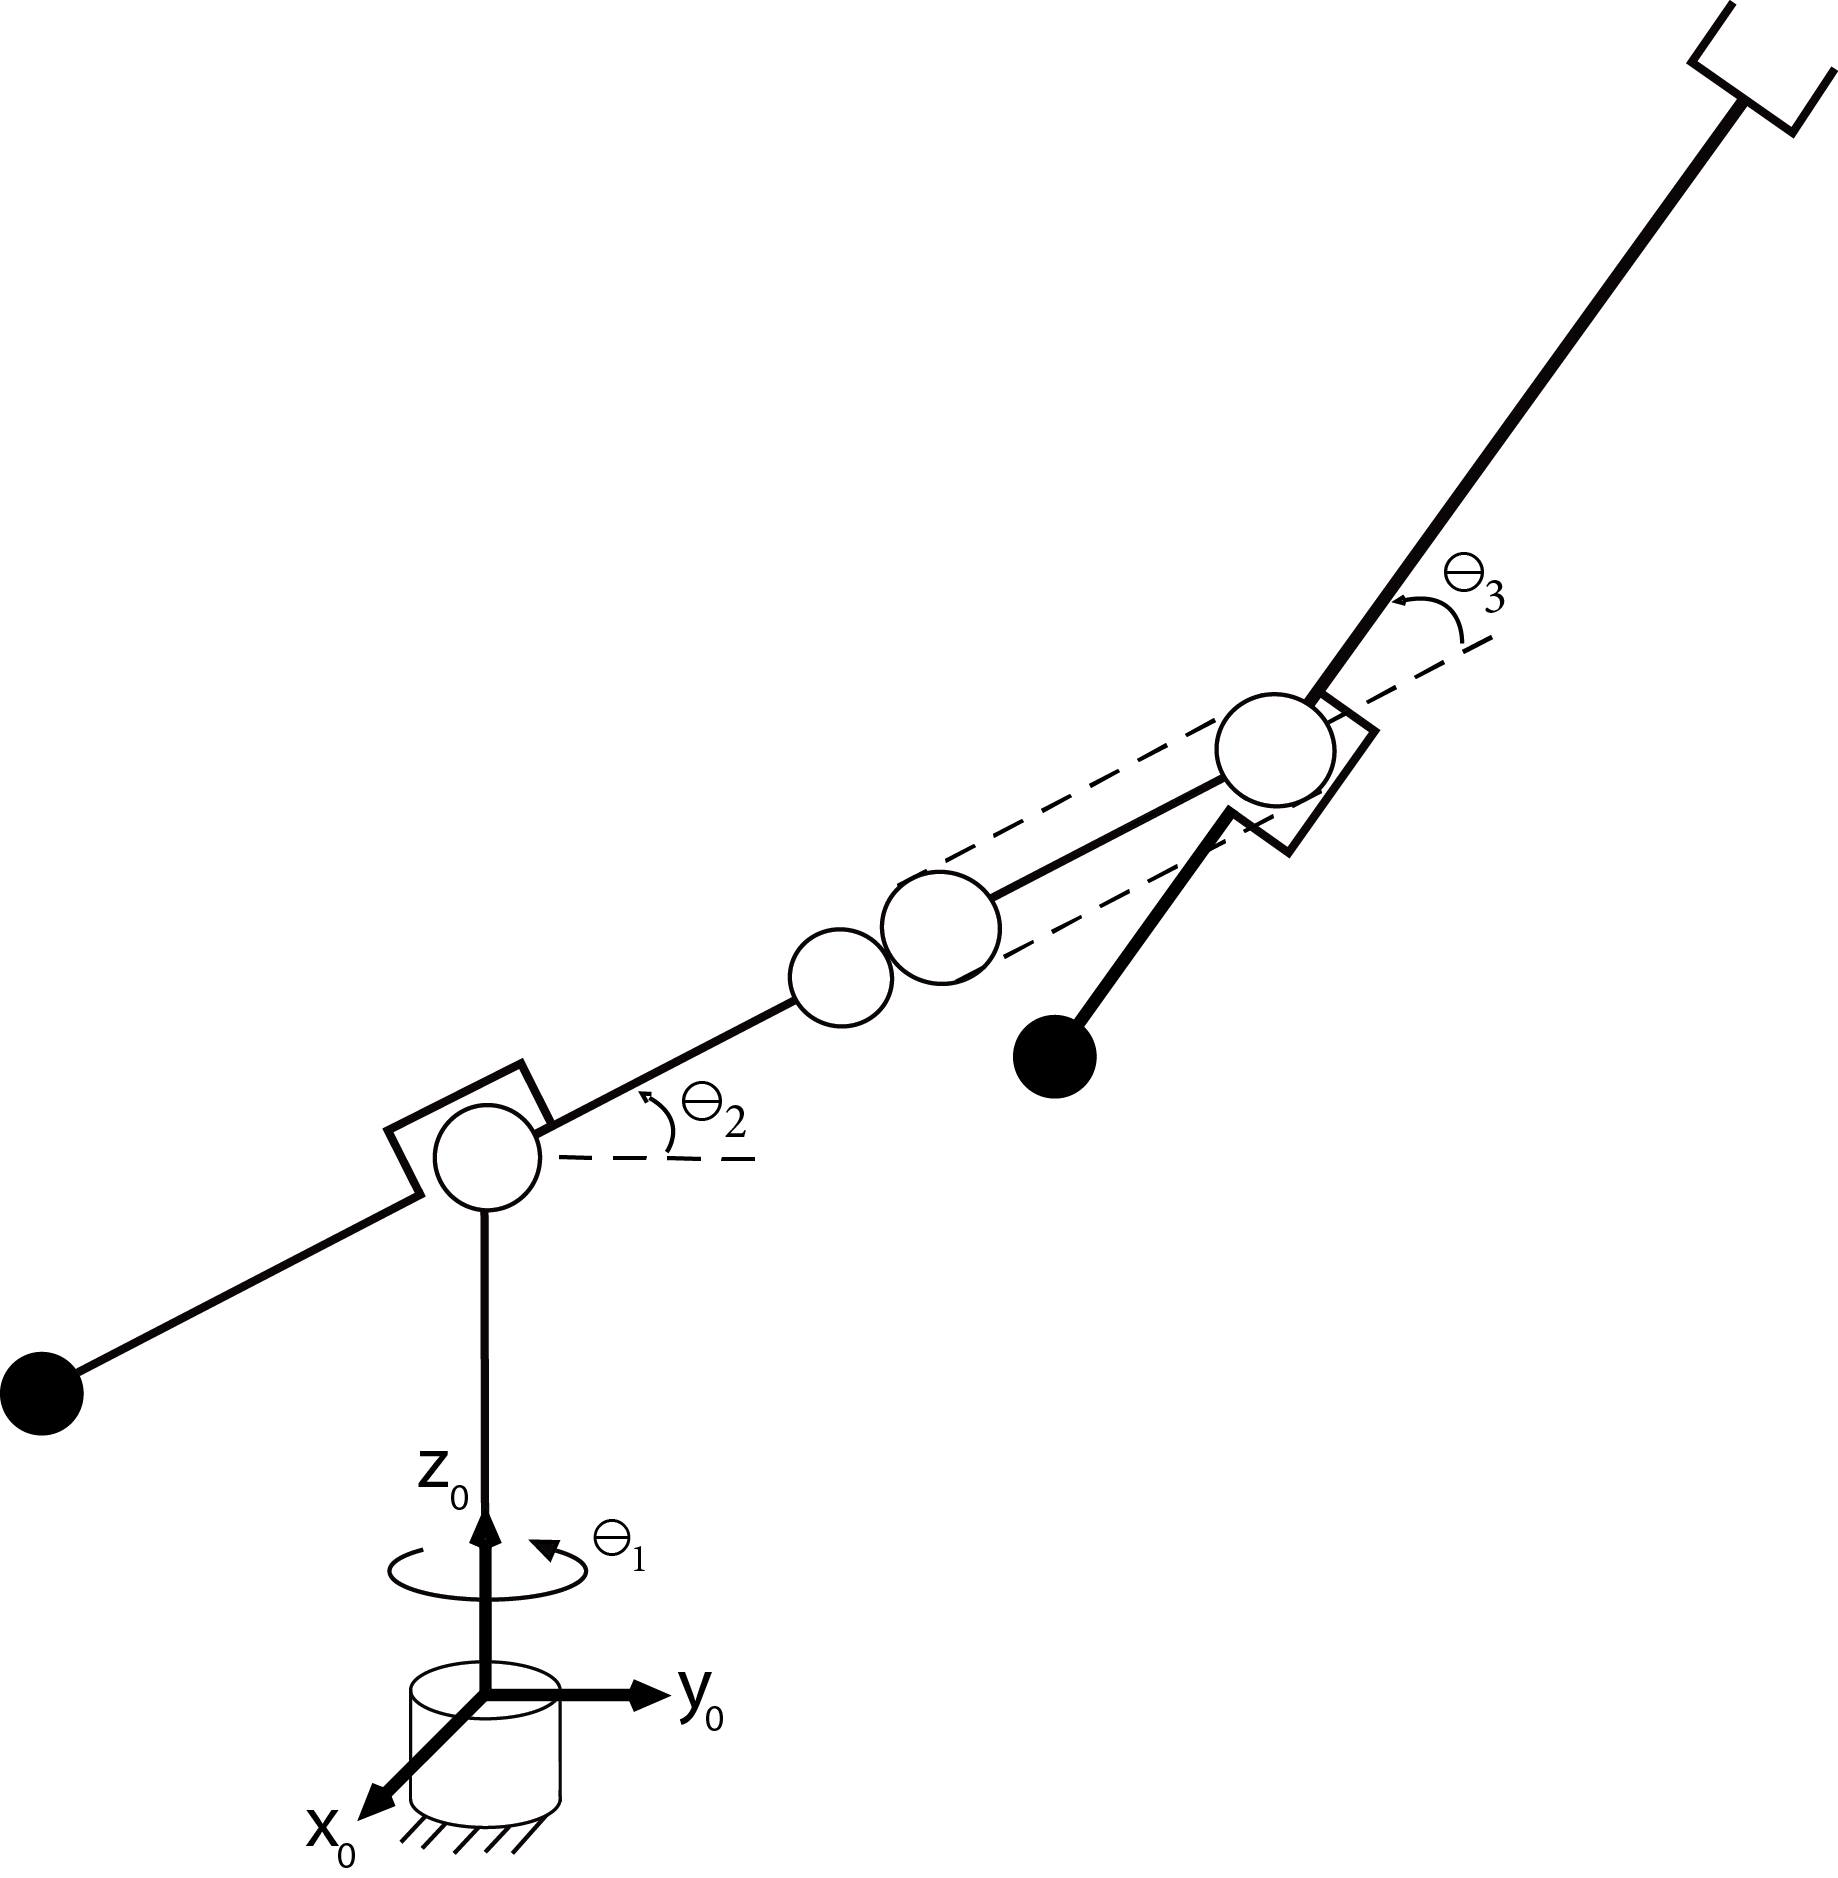
\includegraphics[scale=0.11]{RRR3D.jpg}  
	\caption{Mecanismo RRR espacial}
	\label{fig:RRR3D}
\end{figure}


\begin{equation}
\begin{cases}
D_1 = 0 \\
D_2 = g[ (m_2 l_{g_2} + m_3 l_2  ) \ccos(\theta_2) + m_3 l_{g_3} \ccos(\theta_2 + \theta_3) ]  \\
D_3 = g[ m_3 l_{g_3} \ccos(\theta_2 + \theta_3)  ] \\
\end{cases}
\end{equation} 

Static balancing:
\begin{equation}
\begin{cases}
D_2 = 0 \\
D_3 = 0 \\
\end{cases}
\Rightarrow
\begin{cases}
l_{g_2} = -\frac{l_2 m_3}{m_2} \\
l_{g_3} = 0 \\
\end{cases}
\end{equation}

Static balanced mechanism:
\begin{equation}
\begin{cases}
D_{11} = J_{y_2}\ssin^2(\theta_2) + J_{y_3}\ssin^2(\theta_2+\theta_3) + J_{z_1} + J_{z_2}\ccos^2(\theta_2) + J_{z_3}\ccos^2(\theta_2+\theta_3) + m_3 (l_1 + l_2 \ccos(\theta_2))^2 + \frac{(m_2 l_1 - m_3 l_2 \ccos(\theta_2))^2}{m_2} \\
D_{22} = J_{x_2} + J_{x_3} + m_2 l_2^2 + \frac{l_2^2 m_3^2}{m_2} \\
D_{33} = J_{x_3} \\
D_{12} = D_{13} = 0 \\
D_{23} = D_{33} \\
D_{211} = -\frac{1}{2} \Big( \big( J_{y_2} - J_{z_2} \big) \ssin(2\theta_2) + \big(J_{y_3} - J_{z_3} - m_3 l_2^2 ( 1 + \frac{m_3}{m_2} )\big)\ssin(2\theta_2+2\theta_3)    \Big) \\
D_{311} = \frac{1}{2} \Big( \big(J_{z_3} - J_{y_3} \big)\ssin(2\theta_2+2\theta_3) \Big) \\
D_{111} = D_{122} = D_{133} = D_{222} = D_{233} = D_{322} = D_{333} = 0 \\
D_{112} = - D_{211} \\
D_{113} = - D_{311} \\
D_{123} = D_{212} = D_{213} = D_{223} = D_{312} = D_{313} = D_{323} = 0 \\
\mg = \mzr
\end{cases}
\end{equation}

Coupling 2 discs: \\

Spatial disc models: 
\begin{equation}
\mM\ssh_i = \begin{bmatrix} J_{x_{i+3}} & 0 & 0 \\ 0 & J_{y_{i+3}} & 0 \\ 0 & 0 & J_{z_{i+3}} \end{bmatrix}; \; \mp\ssh_i = \begin{bmatrix} \omega_{x_{i+3}} \\ \omega_{y_{i+3}} \\ \omega_{z_{i+3}} \end{bmatrix}, \; i = 1, 2
\end{equation}

Quasi-velocities constraints:

\begin{equation}
\begin{cases}
\nvct{\vomega_{\scriptscriptstyle 4}}_{\ttB_4} = \nvct{\mone}_{\ttB_4 \rl \ttB_2} \nvct{\vomega_{\scriptscriptstyle 2}}_{\ttB_2} + \begin{bmatrix} \dot{\theta}_3 \\ 0 \\0 \end{bmatrix} \\
\nvct{\vomega_{\scriptscriptstyle 5}}_{\ttB_5} = \nvct{\mone}_{\ttB_5 \rl \ttB_2} \nvct{\vomega_{\scriptscriptstyle 2}}_{\ttB_2} + \begin{bmatrix} \beta\dot{\theta}_3 \\ 0 \\0 \end{bmatrix} \\
\end{cases}
\Rightarrow
\begin{cases}
\omega_{x_4} = \dot{\theta}_2 + \dot{\theta}_3 \\
\omega_{y_4} = (\dot{\theta}_1 \ssin(\theta_2))\ccos(\theta_3) + (\dot{\theta}_1 \ccos(\theta_2))\ssin(\theta_3) \\
\omega_{z_4} = -(\dot{\theta}_1 \ssin(\theta_2))\ssin(\theta_3) + (\dot{\theta}_1 \ccos(\theta_2))\ccos(\theta_3) \\
\omega_{x_5} = \dot{\theta}_2 + \beta\dot{\theta}_3 \\
\omega_{y_5} = (\dot{\theta}_1 \ssin(\theta_2))\ccos(\beta\theta_3) + (\dot{\theta}_1 \ccos(\theta_2))\ssin(\beta\theta_3) \\
\omega_{z_5} = -(\dot{\theta}_1 \ssin(\theta_2))\ssin(\beta\theta_3) + (\dot{\theta}_1 \ccos(\theta_2))\ccos(\beta\theta_3) \\
\end{cases}
\end{equation}

\begin{equation}
\Rightarrow
\underline{\mp}^\circ = 
\begin{bmatrix}
\dot{\theta}_2 + \dot{\theta}_3 \\
\dot{\theta}_1 \ssin(\theta_2+\theta_3) \\
\dot{\theta}_1 \ccos(\theta_2+\theta_3) \\
\dot{\theta}_2 + \beta\dot{\theta}_3 \\
\dot{\theta}_1 \ssin(\theta_2+\beta\theta_3) \\
\dot{\theta}_1 \ccos(\theta_2+\beta\theta_3) \\
\end{bmatrix}
\end{equation}

\begin{equation}
\mC =
\begin{bmatrix}
\mone \\
\displaystyle\frac{\partial \underline{\mp}^\circ}{\partial \mp\ssh}
\end{bmatrix}  =
\begin{bmatrix}
1 & 0 & 0 \\
0 & 1 & 0 \\
0 & 0 & 1 \\
0 & 1 & 1 \\
\ssin(\theta_2+\theta_3) & 0 & 0 \\
\ccos(\theta_2+\theta_3) & 0 & 0 \\
0 & 1 & \beta \\
\ssin(\theta_2+\beta\theta_3) & 0 & 0 \\
\ccos(\theta_2+\beta\theta_3) & 0 & 0 \\
\end{bmatrix} 
\end{equation}

\begin{equation}
\begin{cases}
D'_{11} = D_{11} + J_{y_4}\ssin^2(\theta_2+\theta_2) + J_{y_5}\ssin^2(\beta\theta_2+\theta_2) + J_{z_4}\ccos^2(\theta_2+\theta_2) + J_{z_5}\ccos^2(\beta\theta_2+\theta_2) \\
D'_{22} = D_{22} + J_{x_4} + J_{x_5} \\
D'_{33} = D_{33} + J_{x_4} + J_{x_5} \beta^2\\
D'_{12} = D'_{13} = 0\\
D'_{23} = D_{23} + J_{x_4} + J_{x_5} \beta \\
D'_{211} = D_{211} \\
D'_{311} = D_{311} \\
D'_{111} = D'_{122} = D'_{133} = D'_{222} = D'_{233} = D'_{322} = D'_{333} = 0 \\
D'_{112} = D_{112} +  \frac{1}{4} \Big( \big(J_{y_4} - J_{z_4}\big)\ssin(2\theta_2+2\theta_3) + \big(J_{y_5} - J_{z_5}\big)\ssin(2\beta\theta_2+2\theta_3) \Big) \\
D'_{113} =  D_{113} + \frac{1}{4} \Big( (J_{y_4} - J_{z_4})\ssin(2\theta_2+2\theta_3) + (J_{y_5} - J_{z_5})\ssin(2\beta\theta_2+2\theta_3) \Big) \\
D'_{123} = D'_{212} = D'_{213} = D'_{223} = D'_{312} = D'_{313} = D'_{323} = 0 \\
\end{cases}
\end{equation}

Dynamic balancing:
\begin{equation}
\begin{cases}
D'_{23} = 0 \\
D'_{211} = 0 \\
D'_{311} = 0 \\
D'_{112} = 0 \\
D'_{113} = 0 \\
\end{cases}
\Rightarrow
\begin{cases}
\beta = -\frac{J_{x_3}+J_{x_4}}{J_{x_5}} \\
J_{y_2} = J_{z_2} \\
J_{y_3} = J_{z_3} + m_3 l_2^2 ( 1 + \frac{m_3}{m_2} )\\
J_{y_4} = J_{z_4} \\
J_{y_5} = J_{z_5} \\
\end{cases}
\end{equation}

Dynamic balanced mechanism:
\begin{equation}
\begin{cases}
\tau_1 = k_1 \ddot{\theta}_1 \\
\tau_2 = k_2 \ddot{\theta}_2 \\
f_3 = k_3 \ddot{d}_3 \\
\end{cases}
\end{equation}

Being:
\begin{equation}
\begin{cases}
k_1 = J_{z_1} + J_{z_2} + J_{z_3} + J_{z_4} + J_{z_5} + m_2 l_1^2 + m_3 (l_1^2 + l_2^2) + \frac{l_1^2 m_3^2}{m_2} \\
k_2 =  J_{x_2} + J_{x_3} + J_{x_4} + J_{x_5} + m_3 l_2^2 + \frac{l_1^2 m_3^2}{m_2}\\
k_3 = \frac{(J_{x_3}+J_{x_4})(J_{x_3}+J_{x_4}+J_{x_5})}{J_{x_5}} \\
\end{cases}
\end{equation}

\subsection{3-DOF RRP spatial serial mechanism (SCARA)} \label{S03-2}

\begin{figure}[H]
	\centering
	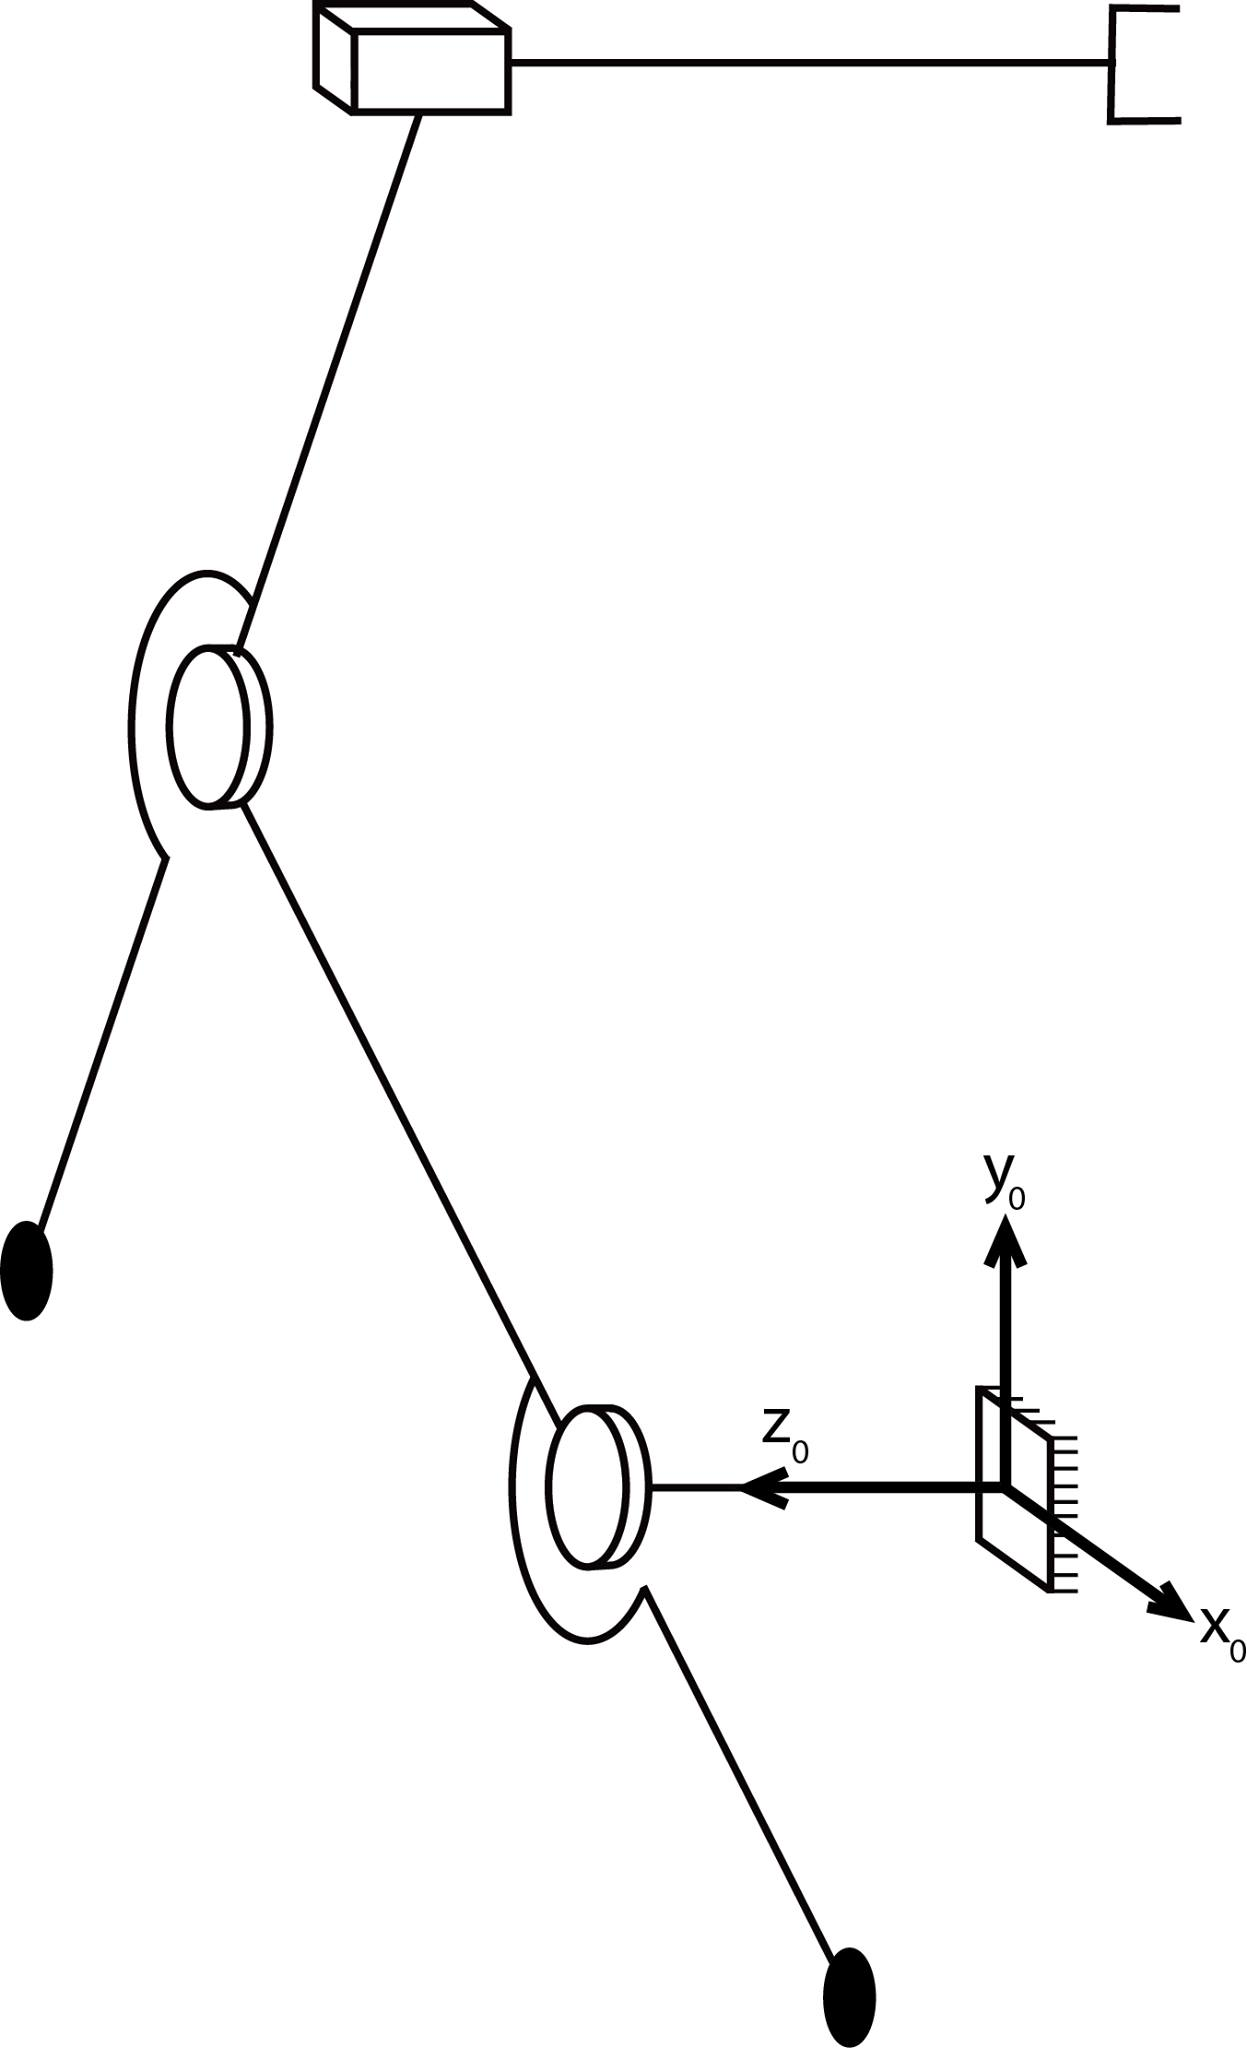
\includegraphics[scale=0.11]{RRP.jpg}  
	\caption{Mecanismo RRP}
	\label{fig:RRP}
\end{figure}


\begin{equation}
\begin{cases}
D_1 = g[ (m_1 l_{g_1} + m_2 l_1 + m_3 l_1 ) \ccos(\theta_1) + m_2 l_{g_2} \ccos(\theta_1+\theta_2) ] \\
D_2 = g[ m_2 l_{g_2} \ccos(\theta_1+\theta_2)  ] \\
D_3 = 0 \\
\end{cases}
\end{equation} 

Static balancing:
\begin{equation}
\begin{cases}
D_1 = 0 \\
D_2 = 0 \\
\end{cases}
\Rightarrow
\begin{cases}
l_{g_1} = -\frac{l_1 (m_2+m_3)}{m_1} \\
l_{g_2} = 0 \\
\end{cases}
\end{equation}

Static balanced mechanism:
\begin{equation}
\begin{cases}
D_{11} = J_{x_1} + J_{x_2} + J_{x_3} + m_2 l_1^2 + m_3 l_1^2 + \frac{l_1^2 (m_2 + m_3)^2}{m_1} \\
D_{22} = J_{x_2} + J_{x_3} \\
D_{33} = m_3 \\
D_{12} = D_{22} \\
D_{13} = D_{23} = 0 \\
\mv\ssh = \mzr \\
\mg\ssh = \mzr
\end{cases}
\end{equation}

Coupling 2 discs: \\

Planar disc models: 
\begin{equation}
\mM\ssh_i = \begin{bmatrix} J_{x_{i+3}} \end{bmatrix}; \; \mp\ssh_i = \begin{bmatrix} \omega_{x_{i+3}} \end{bmatrix}, \; i = 1, 2
\end{equation}

Quasi-velocities constraints:

\begin{equation}
\begin{cases}
\omega_{x_4} = \omega_{x_1} + \dot{\theta}_2 \\
\omega_{x_5} = \omega_{x_1} + \beta\dot{\theta}_2 \\
\end{cases}
\Rightarrow
\begin{cases}
\omega_{x_4} = \dot{\theta}_1 + \dot{\theta}_2 \\
\omega_{x_5} = \dot{\theta}_1 + \beta\dot{\theta}_2 \\
\end{cases}
\Rightarrow
\overline{\mp} = 
\begin{bmatrix}
\dot{\theta}_1 + \dot{\theta}_2 \\
\dot{\theta}_1 + \beta\dot{\theta}_2 \\
\end{bmatrix}
\end{equation}

\begin{equation}
\mC =
\begin{bmatrix}
\mone \\
\displaystyle\frac{\partial \underline{\mp}^\circ}{\partial \mp\ssh}
\end{bmatrix}  =
\begin{bmatrix}
1 & 0 & 0 \\
0 & 1 & 0 \\
0 & 0 & 1 \\
1 & 1     & 0 \\
1 & \beta & 0 \\
\end{bmatrix} 
\end{equation}

\begin{equation}
\begin{cases}
D'_{11} = D_{11} + J_{x_4} + J_{x_5} \\
D'_{22} = D_{22} + J_{x_4} + J_{x_5} \beta^2 \\
D'_{33} = D_{33} \\
D'_{12} = D_{12} + J_{x_4} + J_{x_5} \beta \\
D'_{13} = 0 \\
D'_{23} = 0\\
{\mv'}\ssh = \mzr \\
\end{cases}
\end{equation}

Dynamic balancing:
\begin{equation}
D'_{12} = 0 \Rightarrow \beta = -\frac{J_{x_2}+J_{x_3}+J_{x_4}}{J_{x_5}}
\end{equation}

Dynamic balanced mechanism:
\begin{equation}
\begin{cases}
\tau_1 = k_1 \ddot{\theta}_1 \\
\tau_2 = k_2 \ddot{\theta}_2 \\
f_3 = k_3 \ddot{d}_3 \\
\end{cases}
\end{equation}

Being:
\begin{equation}
\begin{cases}
k_1 = J_{x_1} + J_{x_2} + J_{x_3} + J_{x_4} + J_{x_5} + m_2 l_1^2 + m_3 l_1^2 + \frac{l_1^2 (m_2 + m_3)^2}{m_1} \\
k_2 = \frac{(J_{x_2}+J_{x_3}+J_{x_4})(J_{x_2}+J_{x_3}+J_{x_4}+J_{x_5})}{J_{x_5}} \\
k_3 = m_3 \\
\end{cases}
\end{equation}

%--------------------CONCLUSIONS--------------------%

%\newpage

\section{Conclusions}\label{S04}

This work dealt with a systematic methodology for the adaptive balancing. Two balancing techniques were employed here: the addition of counterweight and counter-rotating disks coupled to the moving links. In addition, the feasibility of the dynamic decoupling for 3 distinct types of serial manipulators was discussed regarding the achievement of such balancing and the complexity level of the modified mechanical structure. The balancing conditions were developed for 3-dof spatial and planar open loop-kinematic chain mechanisms, whose topologies are composed of revolute and prismatic joints. By analysing the necessary conditions, one can notice that the adaptive balancing  brings great benefits for the planar RRR and the spatial RRP. However, for the spatial RRR, in spite of the achievement of the adaptive balancing, the modifications in the mechanical structure cause the increase of the link inertias and the actuator torques, accordingly. Consequently, the authors believe that the discussion provided here might help the designer to choose an adequate topology for a specific application taking advantage of the adaptive balancing whenever it brings no further consequences in terms of the added inertias.

%--------------------ACKNOWLEDGMENTS--------------------%

%\section*{Acknowledgments}


%--------------------BIBLIOGRAPHY--------------------%

% \newpage
\phantomsection 


\begin{thebibliography}{99}


\bibitem{1wijk} 
V. Van der Wijk,
\newblock Shaking moment balancing of mechanisms with principal vectors and moments
\newblock {\em Front. Mech. Eng.}, 8(1): 10--16, 2013.
 
\bibitem{2arakelian}
V. H. Arakelian V. , M. R. Smith,
\newblock Design of planar 3-dof 3-RRR reactionless parallel manipulators
\newblock {\em Mechatronics}, 18: 601--606, 2008. 
 
\bibitem{3seo}
J.-T. Seo, J. H. Woo, H. Lim, J. Chung, W. K. Kim, and B.-J. Yi,
\newblock Design of an Antagonistically Counter-Balancing Parallel Mechanism
\newblock {\em IEEE/RSJ International Conference on
Intelligent Robots and Systems (IROS)}, Tokyo, November 3-7: 2882--2887, 2013. 

\bibitem{4wu}
Y. Wu, C. M. Gosselin,
\newblock Design of reactionless 3-dof and 6-dof parallel manipulators using parallelepiped mechanisms
\newblock {\em IEEE Transactions on Robotics}, 21(5): 821--833, 2005.

\bibitem{5gosselin}
C. M. Gosselin, F. Vollmer, G. C�t�, Y. Wu,
\newblock Synthesis and design of reactionless three-degree-of-freedom parallel mechanisms
\newblock {\em IEEE Transactions on Robotics and Automation}, 20(2): 191--199, 2004.

\bibitem{6wang}
J. Wang, C. M. Gosselin,
\newblock Static balancing of spatial four-degree-of-freedom parallel mechanisms
\newblock {\em Mech. Mach. Theory}, 35: 563--592, 2000.

\bibitem{7wang}
J. Wang, C. M. Gosselin,
\newblock Static balancing of spatial three-degree-of-freedom parallel mechanisms
\newblock {\em Mech. Mach. Theory}, 34: 437--452, 1999.

\bibitem{8alici}
G. Alici, B. Shirinzadeh,
\newblock Optimum Force Balancing with Mass Distribution and a Single Elastic Element for a
Five-bar Parallel Manipulator
\newblock {\em Proceedings of the IEEE International Conference on Robotics and Automation},Taipei, September 14-19: 3666--3671, 2003.

\bibitem{9alici}
G. Alici, B. Shirinzadeh,
\newblock Optimum dynamic balancing of planar parallel
manipulators based on sensitivity analysis
\newblock {\em Mech. Mach. Theory}, 41: 1520--1532, 2006.

\bibitem{10dehkordi}
M. B. Dehkordi, A. Frisoli, E. Sotgiu, M. Bergamasco,
\newblock Modelling and Experimental Evaluation of a Static Balancing Technique for
a new Horizontally Mounted 3-UPU Parallel Mechanism
\newblock {\em International Journal of Advanced Robotic Systems}, 9: 193--205, 2012.

\bibitem{11wang}
K. Wang, M. Luo, T. Mei, J. Zhao, Y. Cao,
\newblock Dynamics Analysis of a Three-DOF Planar Serial-Parallel Mechanism for Active
Dynamic Balancing with Respect to a Given Trajectory
\newblock {\em International Journal of Advanced Robotic Systems}, 10: 23--33, 2013.

\bibitem{12russo}
A. Russo, R. Sinatra, F. Xi,
\newblock Static balancing of parallel robots
\newblock {\em Mech. Mach. Theory}, 40: 191--202, 2005.

\bibitem{13agrawal}
S. K. Agrawal, A. Fattah,
\newblock Gravity-balancing of spatial robotic manipulators
\newblock {\em Mech. Mach. Theory}, 39: 1331--1344, 2004.

\bibitem{14briot}
S. Briot, V. Arakelian, J.-P. Le Baron,
\newblock Shaking force minimization of high-speed robots via centre of mass
acceleration control
\newblock {\em Mech. Mach. Theory}, 57: 1--12, 2012.

\bibitem{15coelho}
T. A. H. Coelho, L. Yong, V. F. A. Alves,
\newblock Decoupling of dynamic equations by means of
adaptive balancing of 2-dof open-loop mechanisms
\newblock {\em Mech. Mach. Theory}, 39: 871--881, 2004.

\bibitem{16moradi}
M. Moradi, A. Nikoobin, S. Azadi,
\newblock Adaptive Decoupling for Open Chain Planar Robots
\newblock {\em Transaction B: Mechanical Engineering}, 17(5): 376--386, 2010.

\bibitem{17arakelian}
V. Arakelian, S. Sargsyan,
\newblock On the design of serial manipulators with decoupled dynamics
\newblock {\em Mechatronics}, 22(6): 904--909, 2012.

\bibitem{18tsai}
J. Chen, D.Z. Chen, L.W. Tsai,
\newblock A Systematic Methodology for the Dynamic Analysis of Articulated Gear-Mechanisms,
\newblock 1990.

\bibitem{19kane}
T. R. Kane, D. A. Levinson,
\newblock {\em {Dynamics, Theory and Applications}}.
\newblock McGraw-Hill series in mechanical engineering. McGraw Hill, 1985.

\bibitem{20altuzarra}
O. Altuzarra, P. M. Eggers, F. J. Campa, C. Roldan-Paraponiaris, C. Pinto, 
\newblock Dynamic Modelling of Lower-Mobility Parallel Manipulators Using the Boltzmann-Hamel Equations
\newblock {\em Mechanisms, Transmissions and Applications}, 31: 157--165, 2015.

\bibitem{21orsino}
R. M. M. Orsino, T. A. H. Coelho, C. P. Pesce, 
\newblock Analytical mechanics approaches in the dynamic modelling of Delta mechanism
\newblock {\em Robotica}, 33(4): 953--973, 2015.

\bibitem{22orsino}
R. M. M. Orsino, A. G. Coutinho, T. A. H. Coelho,
\newblock Dynamic modelling and control of balanced parallel mechanisms.
\newblock Book chapter of {\em Dynamic Balancing of Mechanisms and Synthesizing of Parallel Robots}, Springer, 2016 (in press).

\bibitem{23orsino}
R. M. M. Orsino, T. A. H. Coelho (2015).
\newblock A contribution on the modular modelling of multibody systems.
\newblock Manuscript submitted for publication

\end{thebibliography}


%\end{document}


% \end{multicols}


\end{document}

